% % !TeX program = xelatex
% !TeX spellcheck = es_ES
% !TeX encoding = utf8

\documentclass[onecolumn,10pt,titlepage,a4paper]{article}

\usepackage[a4paper,top=3cm,bottom=2cm,margin=3cm,marginparwidth=1.75cm,headheight=28pt]{geometry}
% Formateo para castellano
%\usepackage[utf8]{inputenc}
\usepackage[spanish,mexico]{babel}
%\usepackage{natbib}


\newcommand{\celsius}{^\circ \mathrm{C}}
\newcommand{\air}{{\mathrm{humo}}}
%Bibliografía

% Simbolos para notas de pie
\usepackage[symbol]{footmisc}
\renewcommand*{\thefootnote}{\fnsymbol{footnote}}

% \renewcommand{\thefootnote}{\fnsymbol{footnote}}
% \footnote[num]{text}

% \pagestyle{myheading}
% \markright{Mi Documento \hfill Mi nombre \hfi}
%
\usepackage{fancyhdr,framed}
\setlength{\headheight}{15.2pt}
\pagestyle{fancy}
\lhead{Elementos Finitos II - 31.92 \\ Patricio Whittingslow -- 55423}
\chead{TP 2}


%\usepackage{subcaption}

% Para el entorno align


% Multiples columnas para glosario
\usepackage{multicol}

%Figuras y subtitulos
\usepackage{graphicx}
\usepackage{caption,subcaption}
\usepackage{hyperref}
\hypersetup{
    colorlinks,
    citecolor=black,
    filecolor=black,
    linkcolor=black,
    urlcolor=black
}
\usepackage[utopia,expert]{mathdesign} %Opcion "expert" para no romperme las smallcaps de helvetica. 
\usepackage{amsmath}

\newcommand{\rmfont}[1]{{\fontfamily{ptm}\selectfont%
		#1}}
\newcommand{\rmfontbf}[1]{{\fontfamily{ptm}\selectfont%
		\textbf{#1}}}
\newcommand{\rmfontsc}[1]{{\fontfamily{ptm}\selectfont%
		\textsc{#1}}}
    
\newcommand{\Matlab}{\rmfont{\sc Matlab}}
    \newcommand{\Adina}{{\sc ADINA}}
    \newcommand{\refp}[1]{(\ref{#1})}
    \newcommand{\unspace}{\!\!\!\!\!\!\!\!\!\!\!\!\!\!\!\!\!\!\!\!}
    \newcommand{\ms}{\ \ \ } %Matrix Spacing
    \newcommand{\di}{\textrm{d}}
    \newcommand{\jac}{\rmfontbf{J}}
    \newcommand{\Djac}{|\;\jac\;|}
    \newcommand{\dNi}{\di N_i}
    \newcommand{\sigmab}{\boldsymbol{\sigma}}
    \newcommand{\varepsilonb}{\boldsymbol{\varepsilon}}
    \newcommand{\Phib}{\boldsymbol{\Phi}}
    \newcommand{\CPhi}{\boldsymbol{\{ } \Phi \boldsymbol{\} }}
    \newcommand{\Mme}[1]{\boldsymbol{[}\mathbf{#1} \boldsymbol{]}}
    \newcommand{\Rme}[1]{\boldsymbol{\lfloor}\mathbf{#1} \boldsymbol{\rfloor}}
    \newcommand{\Cme}[1]{\boldsymbol{\{ }\mathbf{#1} \boldsymbol{\}} }
    \newcommand{\MB}{\Mme{B}}
    \newcommand{\MN}{\Mme{N}}
    \newcommand{\ME}{\Mme{E}}
    \newcommand{\Mk}{\Mme{k}}
    \newcommand{\MA}{\Mme{A}}
    \newcommand{\radial}{r}
    \newcommand{\eff}{f}
%Helvetica
\renewcommand{\familydefault}{\sfdefault}
\usepackage[scaled=1]{helvet}
\usepackage[format=plain,
            labelfont={bf,it},
            textfont=it]{caption}
%\usepackage[T1]{fontenc}
%--------------------------------------


\usepackage{siunitx}
\newcommand{\glossentry}[2]{$#1\ $ \indent #2 \par \vspace{.4cm} }
\newcommand{\adm}{\textrm{adm}}
\renewcommand\thepart{\Alph{part}}

\title{Informe Técnico - ITBA}

\author{Patricio Whittingslow}
%========================> Comienza Documento
\begin{document}
\begin{titlepage}
	\centering
	
	{ \large Instituto Tecnológico de Buenos Aires  \par }
	\vspace{2cm}
	{\Large \scshape Elementos Finitos II - 31.92 \par}
	\vspace{2cm}
	{\Huge \scshape Estudio técnico de un satélite de titanio utilizando el método de elementos finitos\par }
	\vspace{.5cm}
	{\Large  \par}
	\vspace{2cm}
	{\large \bf Autor \par}
	\vspace{.5cm}
	\textsc{\large Patricio Whittingslow -- 55423}
	\vspace{2cm}
	{\par \large Fecha de realización: \today \par}
	\vspace{1cm}
	{\large Fecha de entrega: .......................................\par}
	\vspace{\fill}
	{\large Firma del docente: .......................................}
	\vspace{\fill}
	\begin{figure}[htb!]
		\centering
		
\includegraphics[width=6cm]{fig/logoitba.png}
	\end{figure}
\end{titlepage}




\begin{multicols}{2}
	\section*{Glosario}
	\glossentry{\Cme{R}}{Vector de cargas térmicas.}
	\glossentry{\Mme{K}}{Matriz de conductividad.}
	\glossentry{\Mme{C}}{Matriz de capacidad térmica.}
	\glossentry{\Cme{T}}{Vector de Temperaturas.}
\end{multicols}

%\setcounter{section}{-1}
\newcommand{\xx}{{\mathrm{xx}}}
\newcommand{\xc}{{\mathrm{xc}}}
\newcommand{\cc}{{\mathrm{cc}}}
\newcommand{\sx}{{\mathrm{x}}}
\newcommand{\scc}{{\mathrm{c}}}
%\tableofcontents

\section*{Objetivo}
Se va efectuar un estudio térmico de un satélite ubicado en el espacio profundo. El problema será resuelto mediante el método de elementos finitos.

\section*{Hipótesis}
\begin{itemize}
	\item Material isótropo y homogéneo
	\item Propiedades sin dependencia de variables termodinámicas
\end{itemize}


\section*{Método}

El satélite será modelado como un cubo de titanio macizo. Este se encuentra en el vacío del espacio profundo, el cual tiene una temperatura $T_{\mathrm{CMBR}}=2,7$ K. El modelo se simplifica tomando solo una octava parte del satélite, aprovechando la doble simetría. 

El satélite tiene lados de longitud $L=0,8$m. Las propiedades del titanio son las siguientes:
\begin{itemize}
	\item $c_p = 528 \si{\joule \per \kilogram \per \kelvin}$
	\item $\rho = 4500\si{\kilogram \per \meter \cubed }$
	\item $k = 17 \si{\watt \per \meter \kelvin}$
\end{itemize}

Las condiciones de operación son las siguientes
\begin{itemize}
	\item El medio del satélite opera a 300K.
	\item El satélite genera $q_{G}=2\si{\kilo \watt \per \meter \cubed}$
	\item El calor radiado tomando en cuenta el factor de forma queda $q_{r}=\SI{1,417e-8}{\watt \per \meter \squared \per \kelvin^4} \cdot \left( T^4 - T^4_{\mathrm{CMBR}} \right)$
\end{itemize}

Para la resolución se dividió el satélite en 2744 elementos H8.

Las condiciones de borde son las siguientes
\begin{itemize}
	\item Se fija el punto medio del satélite a 300K
	\item Las superficies expuestas del satélite intercambian calor con el entorno según la ecuación mencionada anteriormente
\end{itemize}

Comienza la iteración  y termina una vez llegado a un error aceptable (ecuación \ref{ec:error})
\begin{equation}\label{ec:error}
	e_{\mathrm{convergencia}}=\frac{||\CT^{n+1}-\CT^{n}||}{||\CT^{n}||} < 10^{-7}
\end{equation}

Se utiliza el método iterativo para resolver la radiación con relajación

\begin{equation}
\begin{cases}
	\Cme{T_\sx}^{n+1}_{\mathrm{unrelaxed}} =  \Mme{K_\xx} ^{-1}  \left(\Cme{R_\sx}^{n} - \Mme{K_\xc} \Cme{T_\scc}^{n}\right)\\
	\CR^{n} = \Cme{R_{\mathrm{generado}}}+ \Cme{R_{\mathrm{rad}}}^{n} \\
	\Cme{T}^{n+1} = \Cme{T}^n + \frac{1}{k_R} \cdot \left( \Cme{T}^{n+1}_{\mathrm{unrelaxed}} - \Cme{T}^{n} \right)
\end{cases}
\end{equation}
donde $\Cme{R_{\mathrm{rad}}}^{n}$ está en función de la temperatura de la superficie a temperatura $\Cme{T}^{n}$ y donde $k_R$ es el factor de relajación. Para los casos resueltos se utilizó $k_R=16$.

\section*{Resultados}
La figura \ref{fig:perfil15} muestra el perfil de temperaturas dentro del satélite en su interior mientras que la figura \ref{fig:perfilsurf15} muestra el perfil superficial del satélite. 
\begin{figure}[htb!]
	\centering
	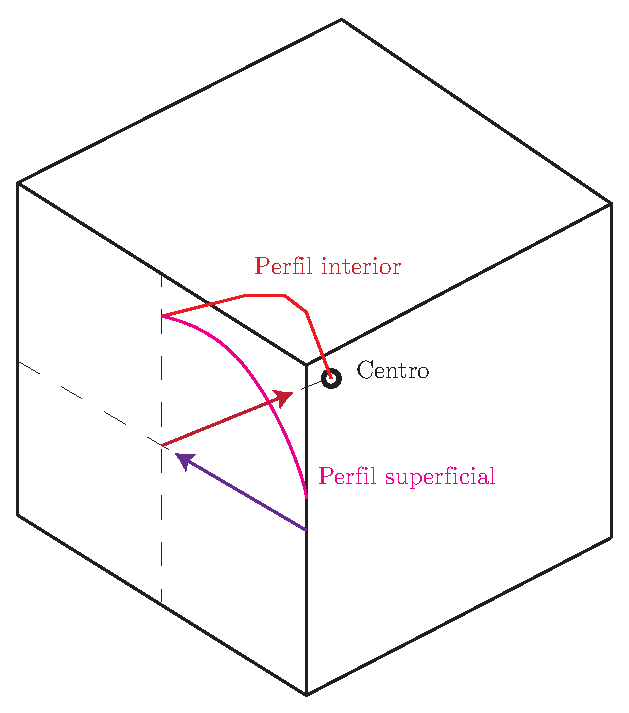
\includegraphics[width=0.4\textwidth]{fig/modelo.eps}
	\caption{Orientación de gráficos.}
	\label{fig:modelo}
\end{figure}


En la figura \ref{fig:perfilsurf15} se ve como un sistema simple como un cubo puede devolver perfiles de temperatura que pueden no tener una razón de ser inmediatamente aparente. En la figura \ref{fig:perfilsurf15} podemos ver como los bordes están mas fríos que el centro de la cara radiadora. Es razonable pensar que los bordes tienen más superficie que los rodea y por ende terminan radiando más que el centro de la cara que se encuentra rodeada por masa. Sin embargo también entra en juego el medio del satélite, el cual se encuentra a una temperatura (300K) más fría que el resto del satélite. El centro se encuentra más cerca a la parte de la cara más caliente, sin embargo, su efecto enfriador se extiende hasta 25\% del camino a la cara, como se puede ver en la figura \ref{fig:perfil15}. 

Resolviendo para las cargas desconocidas se obtiene que el satélite pierde 10 watts en su centro.
\begin{figure}[htb!]
	\centering
	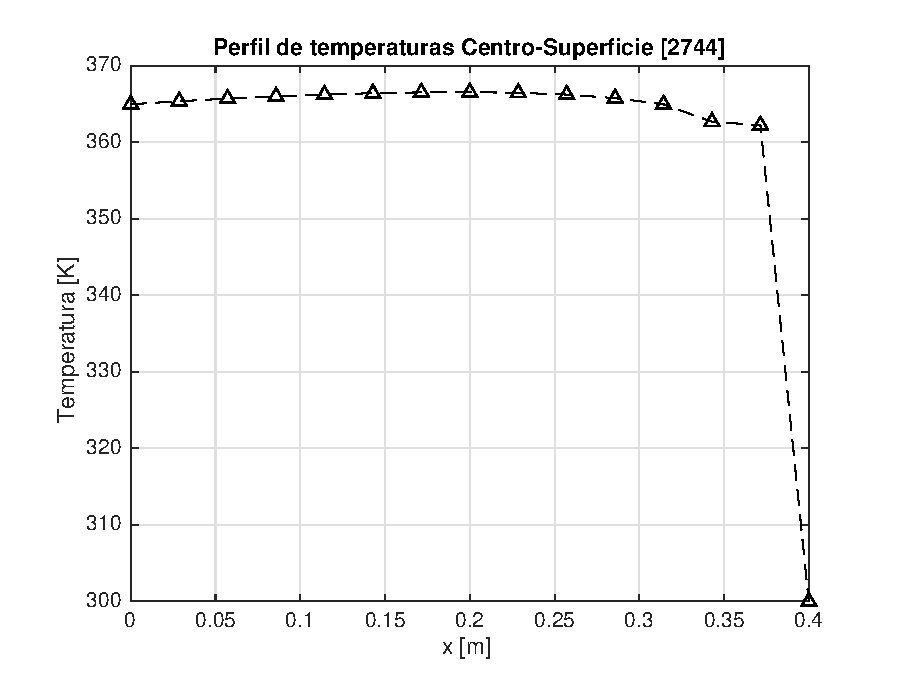
\includegraphics[width=0.8\textwidth]{fig/perfil13.eps}
	\caption{Perfil de temperaturas para 15 divisiones de lado. El gráfico comienza sobre el medio de la superficie del satélite ($x=0$) y continúa hasta llegar al centro del satélite ($x=0,4$m).  }
	\label{fig:perfil15}
\end{figure}
\begin{figure}[htb!]
	\centering
	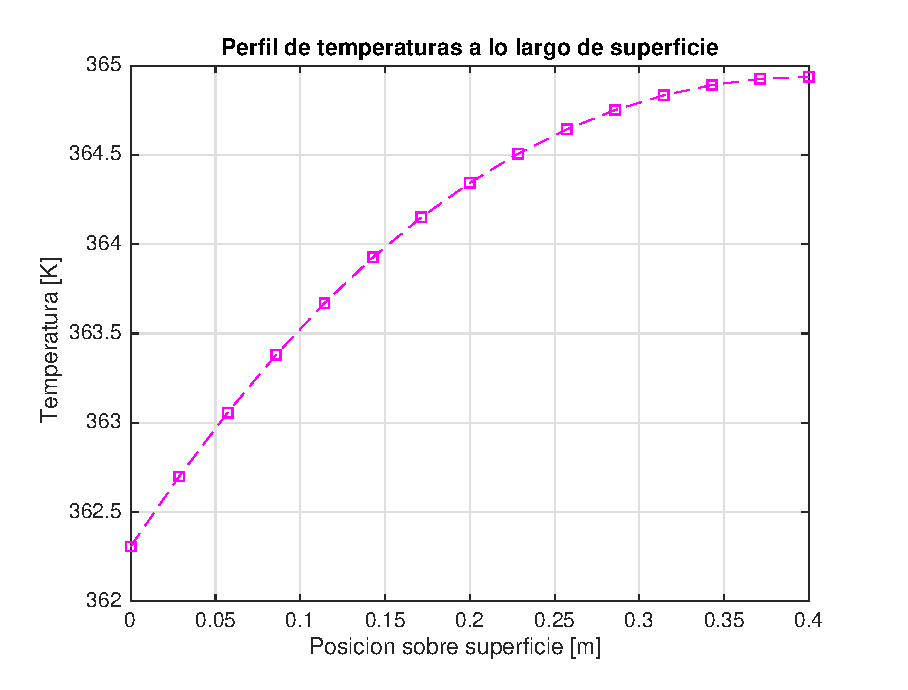
\includegraphics[width=0.8\textwidth]{fig/perfilsurf15.eps}
	\caption{Perfil de temperaturas de la superficie para 15 divisiones de lado. }
	\label{fig:perfilsurf15}
\end{figure}

\begin{figure}[htb!]
	\centering
	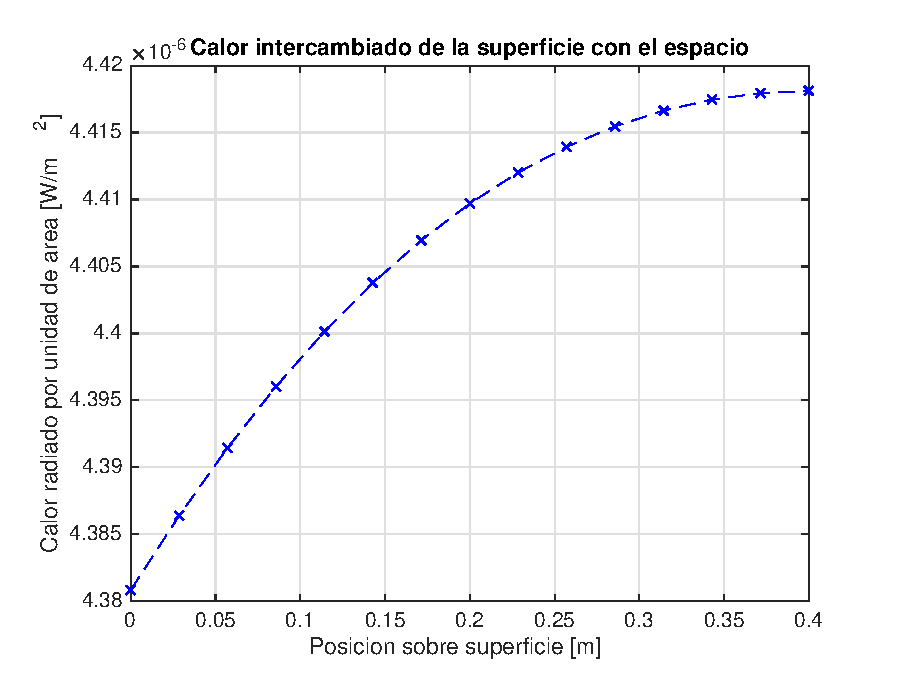
\includegraphics[width=0.8\textwidth]{fig/calorint15.eps}
	\caption{Calor intercambiado de la superficie con el espacio. 15 divisiones de lado.}
	\label{fig:calor}
\end{figure}

\section*{Conclusión}
En conclusión, el satélite tendría que estar evacuando calor en su centro para mantener la temperatura de 300 grados kelvin. Esto se podría lograr usando un enfriador (\ref{fig:cryocooler}) o bien optando por una solución \textit{pasiva} y aumentando la superficie radiante del satélite. 

Si se quiere resolver el problema de forma pasiva fijando el calor generado por unidad volumen se llega a que se tiene que reducir el volumen del satélite. Aunque el satélite se acerque a una forma esférica\footnote{Una esfera es la forma maciza más eficiente de radiar calor dado un volumen fijo.} se tiene que el régimen estacionario de una esfera que genera 2 kW/m$^3$ está a 328 Kelvin. 

\begin{figure}[htb!]
	\centering
	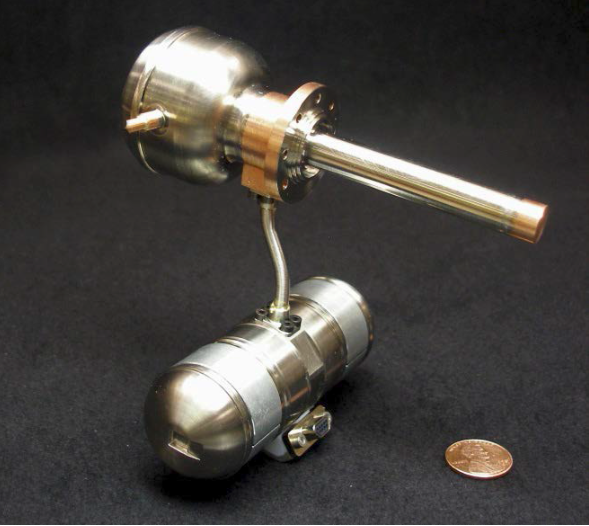
\includegraphics[width=0.8\textwidth]{fig/cryocooler.png}
	\caption{Microenfriador para aplicaciones aerospaciales (Lockheed Martin). }
	\label{fig:cryocooler}
\end{figure}


%\bibliography{labibliografia} % Indica archivo
%\bibliographystyle{plainnat} 

\end{document}